\section{Fachliche Konzeption}

\subsection{Ziel- Nutzergruppe}

Primäre Zielgruppen sind die Technologiestiftung Berlin und der Verein Flussbad Berlin. Des weiteren sind die erhobenen Daten für Dritte zugänglich und relevant. Die TSB ist als Auftraggeber von besonderer Bedeutung. Der VFB ist als Partner für die Messstandorte besonders für die Erprobungsphase wichtig. Der Prototyp muss eventuell auch an die Gegebenheiten des vom VFB zur Verfügung gestellten Standortes angepasst werden.

\subsection{Inhaltlicher Aufbau/Komponenten}\label{subsec:con_strct_comp}

\subsubsection{Messstation}
Die Messstation besteht aus einem Arduino Uno als Basisplattform (siehe~\autoref{fig:ardoinoUno}) und einem Dragino-Shield für die Kommunikation mittels des LoRaWAN Protokoll (siehe~\autoref{fig:draginoShield}). Für die Erfassung der Wasserdaten kommen Sensoren für pH-Wert, Trübheit, sowie Temperatur zum Einsatz.\newline
Der Arduino und das Dragino-Shield sind in einem witterungsbest\"andig Gehäuse untergebracht. Das Gehäuse besitzt mindestens die Schutzklasse IP65, damit die Komponenten ausreichend gegen Nässe geschützt sind. Die Sensoren sind außerhalb des Gehäuses und durch wasserfeste Kabeldurchführungen verbunden. Die Energieversorgung der Messstation wird über eine externe Stromversorgung sichergestellt.

\begin{figure}[H]
	\centering
	\begin{minipage}[t]{0.45\linewidth}
		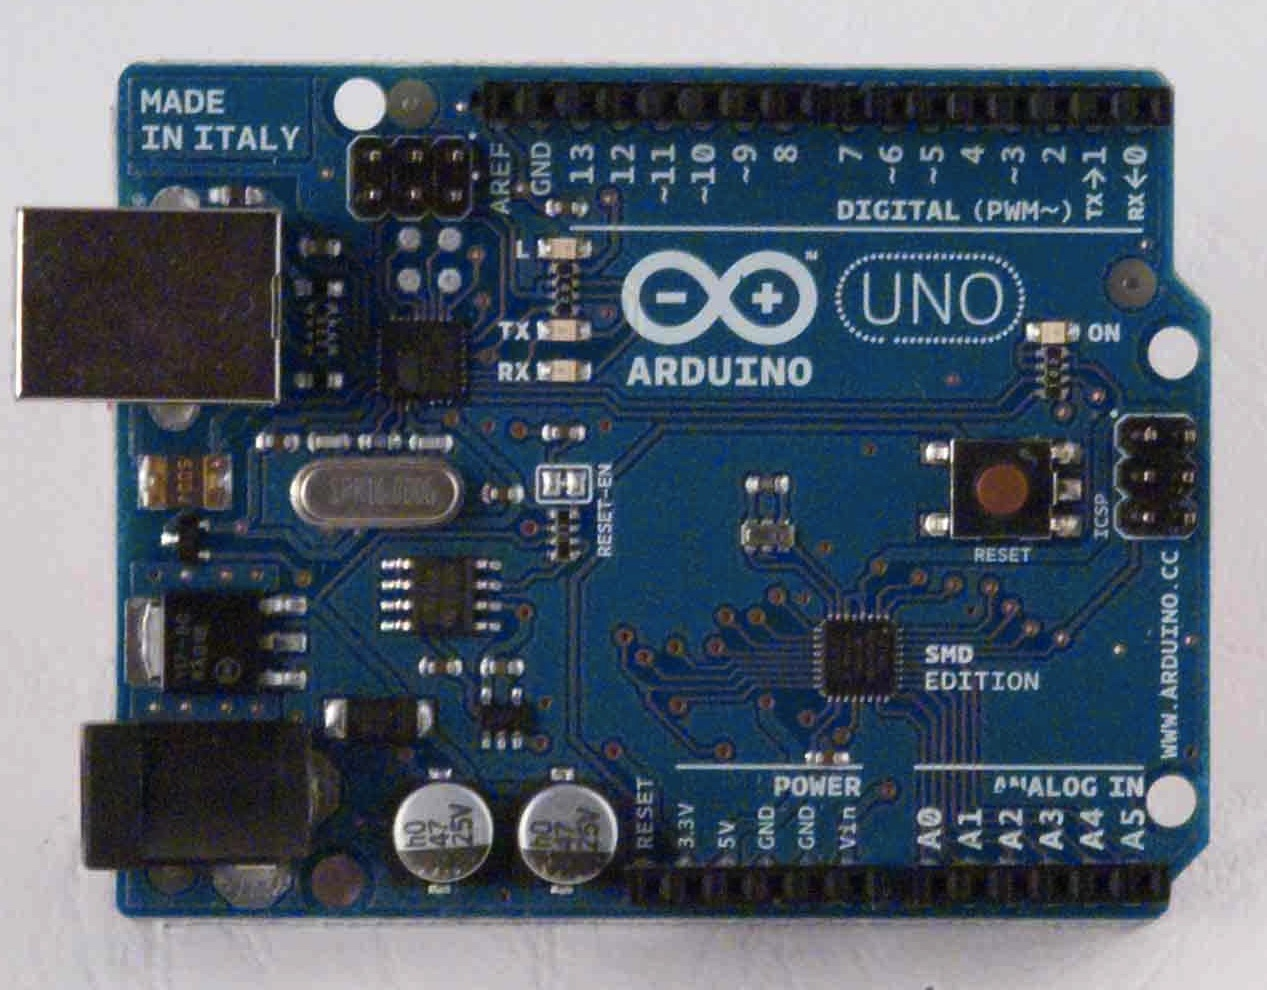
\includegraphics[width=7cm]{figures/ArduinoUnoSMDFront.jpg}
		\caption{Arduino Uno der SMD Variante. Veröffentlicht auf \href{https://www.arduino.cc/en/Main/ArduinoBoardUnoSMD}{Arduino.cc}}
		\label{fig:ardoinoUno}
	\end{minipage}
	\hfill
	\begin{minipage}[t]{0.45\linewidth}
		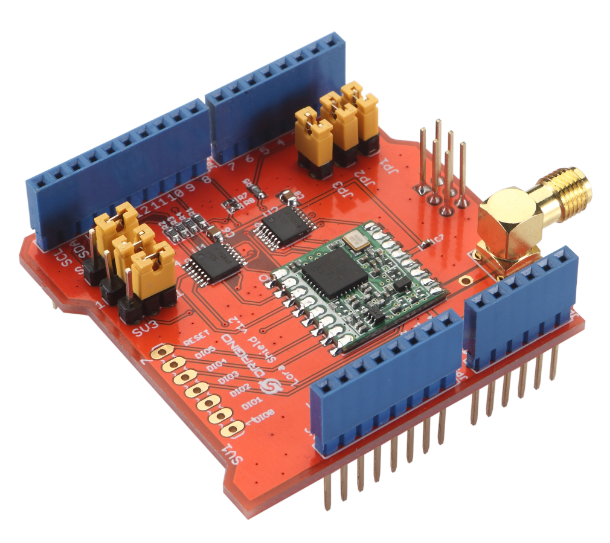
\includegraphics[width=7cm]{figures/LoraShield-1.png}
		\caption{Dragino LoRa Shield. Veröffentlicht auf \href{http://www.dragino.com/products/lora/item/102-lora-shield.html}{dragino.com}}
		\label{fig:draginoShield}
	\end{minipage}
\end{figure}

\subsubsection{Datenbankserver}
Für das Speichern der empfangenen Daten kommt ein MySQL Datenbanksystem zum Einsatz. Hier werden sämtliche von TTN übermittelten Daten abgelegt. Die Daten werden nicht im Rohformat gespeichert, sondern soweit aufbereitet, sodass nach ihrer Auswertung Metadaten, Messwert und Node strukturiert in der Datenbank liegen.

\subsubsection{Datenmodell}
\begin{figure}[H]
	\centering
	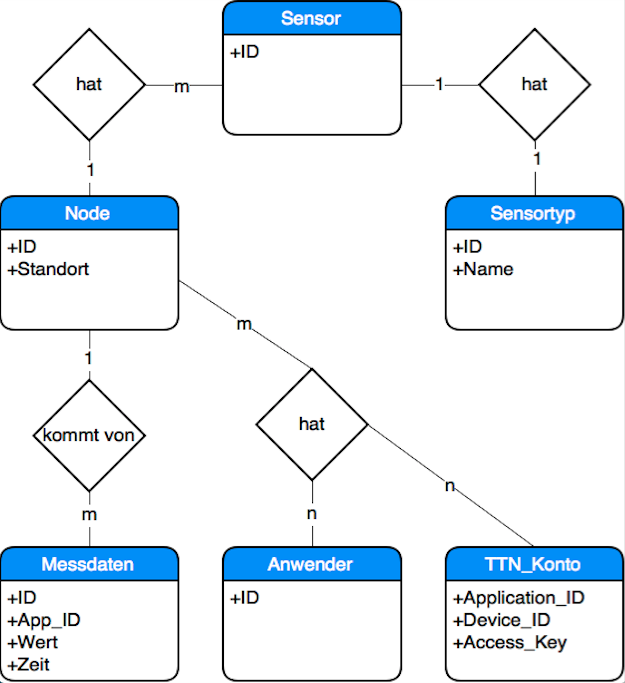
\includegraphics[width=6cm]{figures/dbmodel.png}
	\caption{Datenbankmodel}
	\label{fig:dbModel}
\end{figure}

\subsubsection{Webserver}
Der Webserver besitzt folgende Funktionalitäten:
\begin{itemize}
	\item Eine Schnittstelle für TTN, um die Daten von dort zu empfangen. Die Daten werden im JSON Format übertragen.
		  Bei Empfang werden diese dann in der Datenbank gespeichert. Da es sich um eine URL basierte Schnittstelle handelt, werden nur POST-request's verarbeitet.
		  So wird verhindert das durch ein Aufrufen der URL mittels eines Browsers fremde Daten hinzufügt werden.
	  \item Eine Schnittstelle, die f\"ur das Abrufen der gespeicherten Daten verantwortlich ist. Die Daten werden mittels eines GET-request und Parametern in der Abfrage bereitgestellt. Ein einfaches Web-Formular dient als Generator zum erstellen der URL.
\end{itemize}
Desweiteren dient der Webserver zur Präsentation des Projektes.

\subsubsection{Use Case}
\begin{figure}[H]
	\centering
	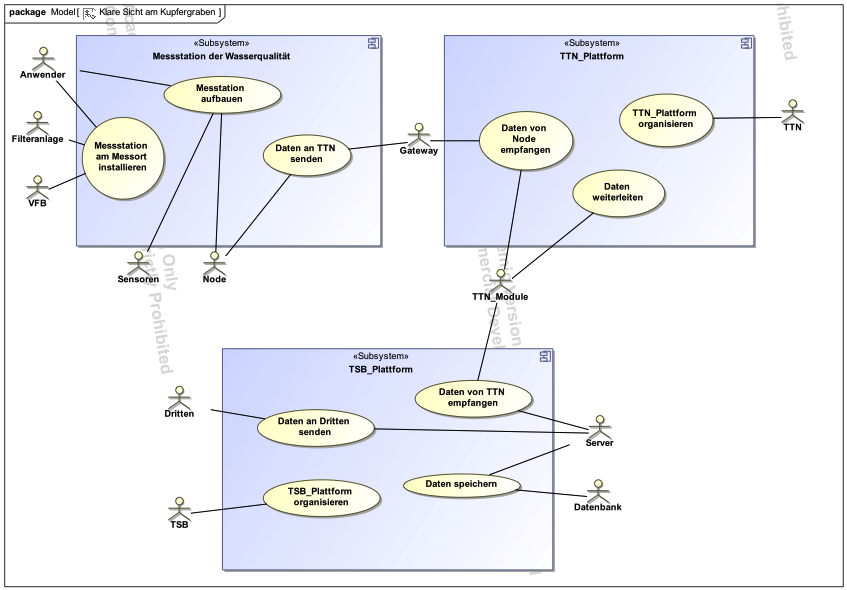
\includegraphics[width=10cm]{figures/use-case.png}
	\caption{Use-Case model}
	\label{fig:useCase}
\end{figure}
